% !TEX root = ../foresight.tex

\section{Introduction}

\begin{figure}
    \centering

    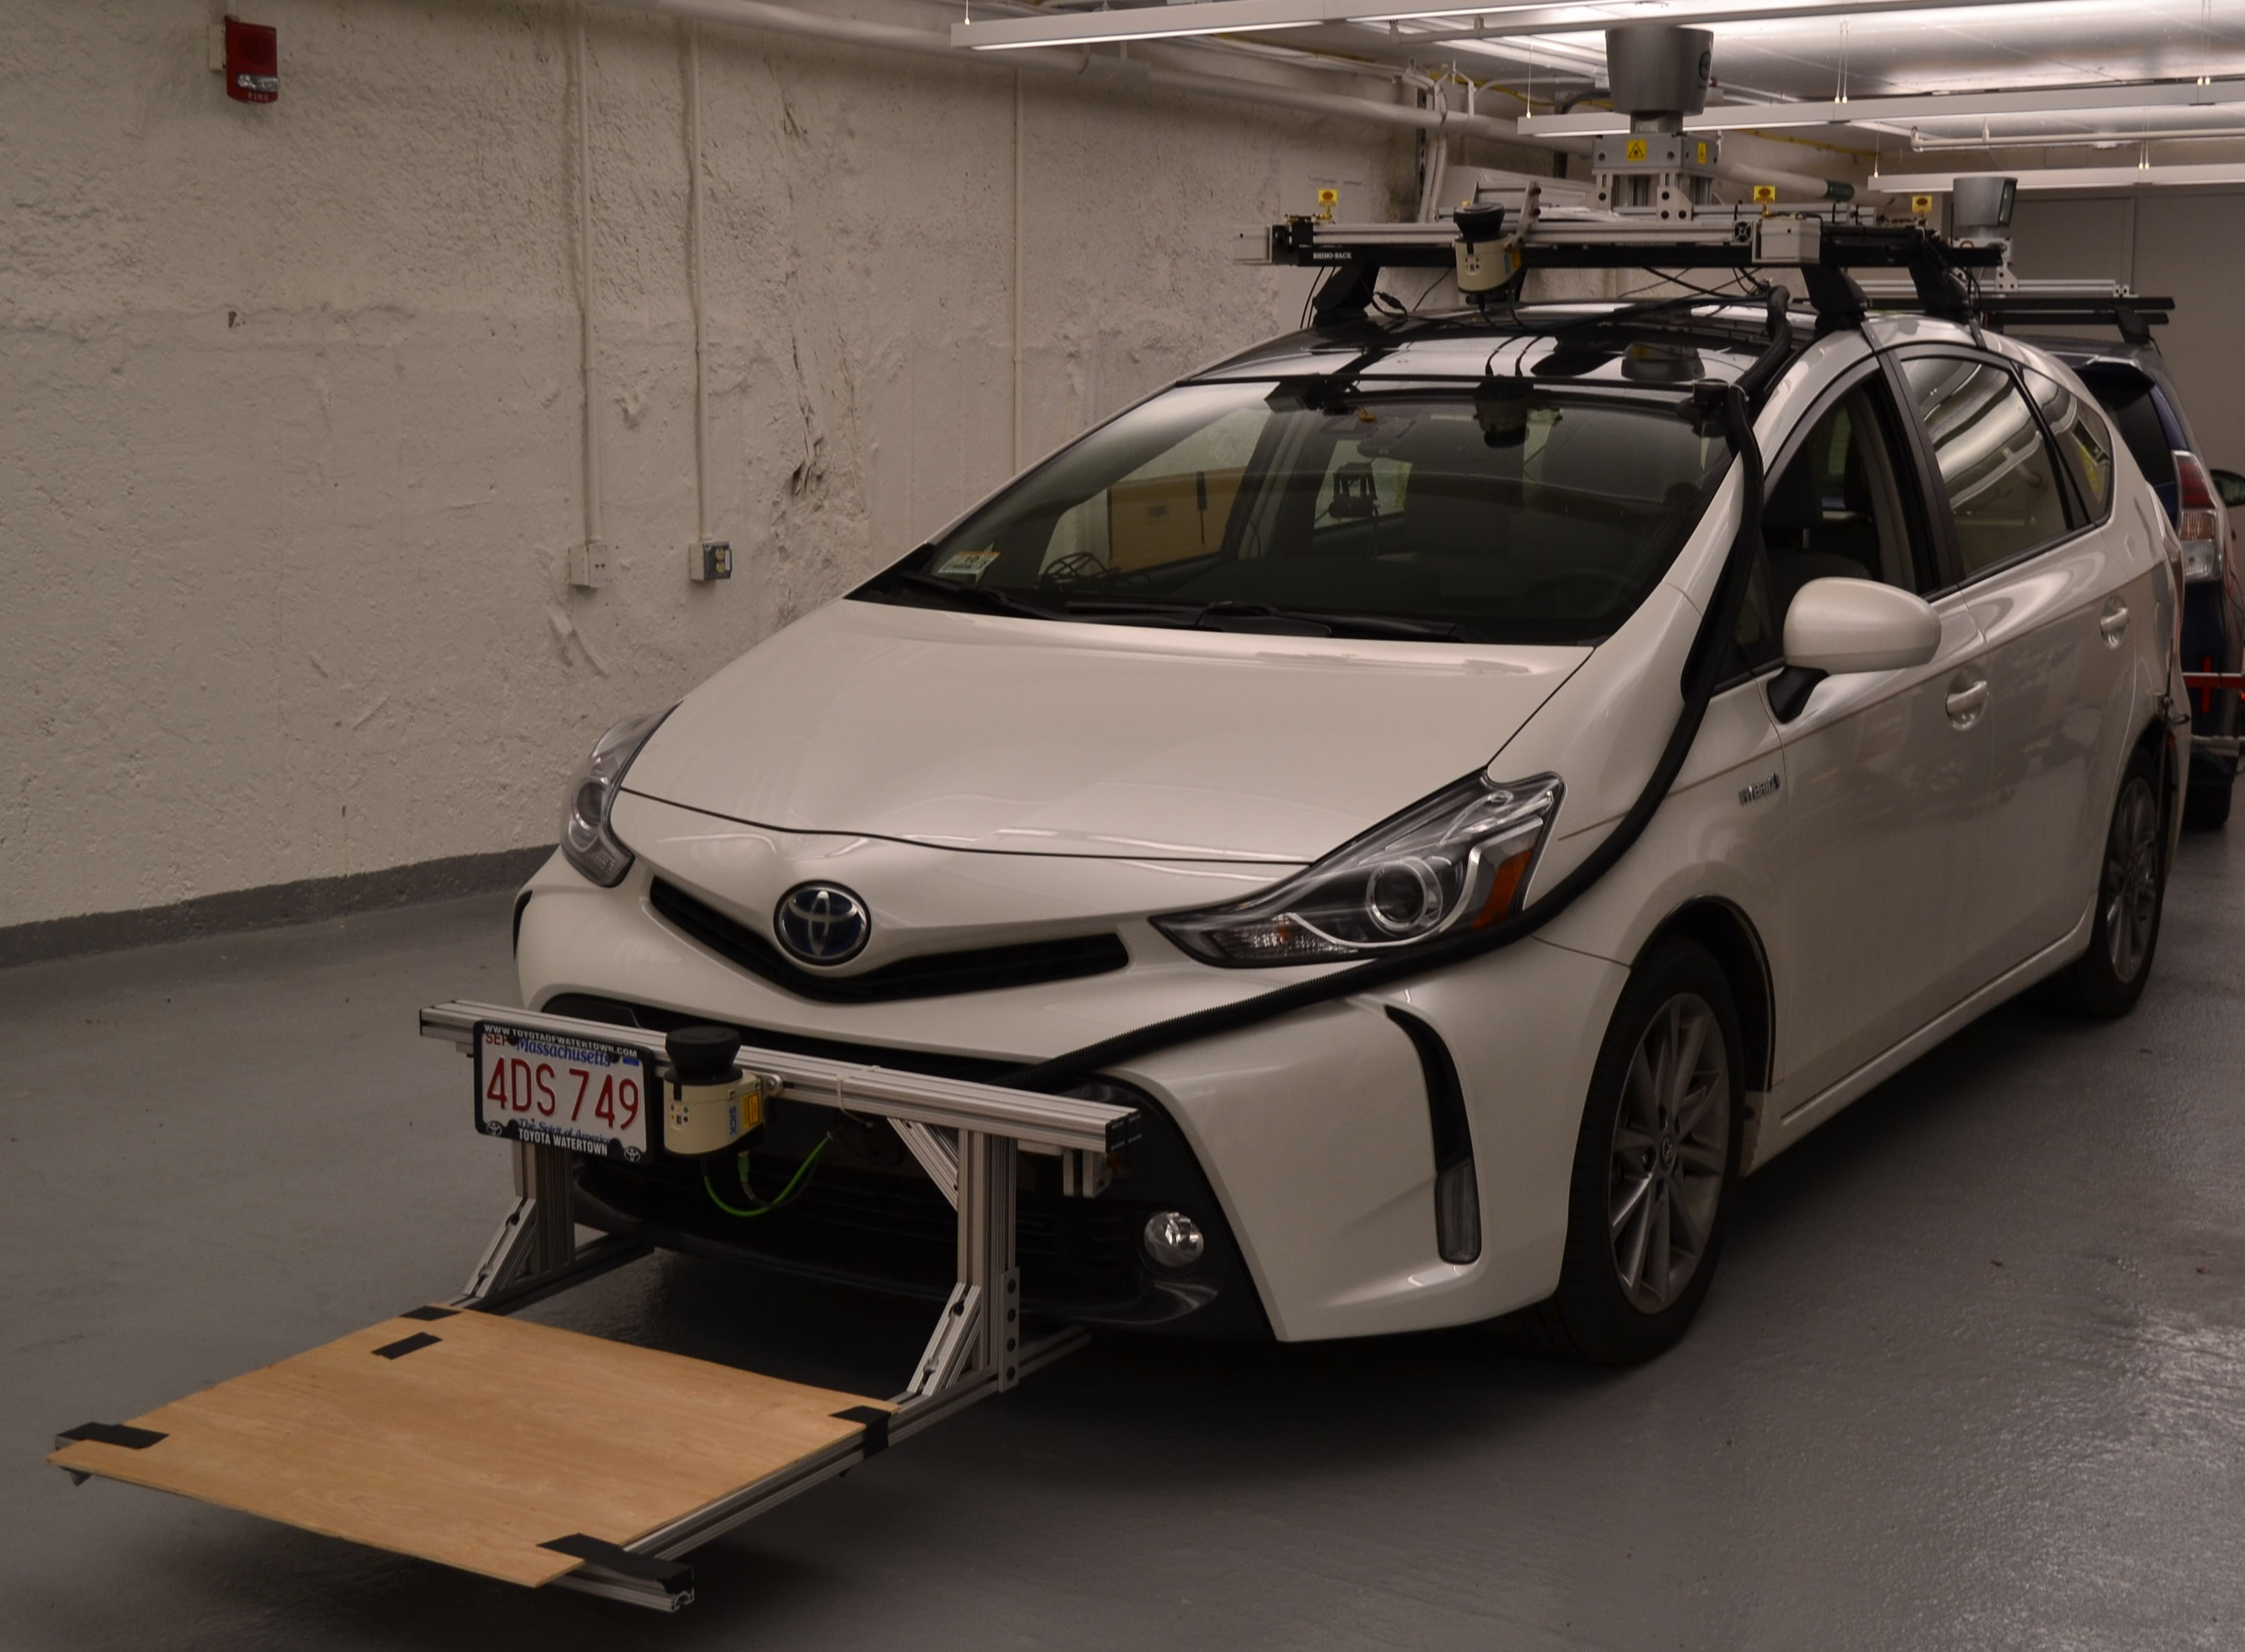
\includegraphics[angle=90, width=0.6\linewidth]{car}

\end{figure}

Globally, over 3000 people die \emph{every day} \cite{ASIR2016} in vehicle-related accidents and over one hundred thousand are injured or disabled on average.
% Worse still is that this number is continuing to increase \cite{NSC2016Fatality}.
In the United States, over 90\% of these accidents were due to human error \cite{NHTSA_crash_stats}.
This has resulted in the continued development of advanced safety systems by commercial car manufacturers.
%Safety systems in automobiles are undergoing rapid development to address the fact troubling continued increase in traffic injuries and fatalities \cite{NSC2016Fatality}. 
For example, systems exist to automatically brake in the case of unexpected obstacles \cite{Toyota_patent}, maintain a car in a lane at a given speed \cite{bradley2016tesla}, alert users of pedestrians, signage, and other vehicles on the roadway \cite{Dagan_IVS_2004}. These systems will make our cars safer and eventually autonomous.
However many accidents are due to blind spots, for example when a vehicle takes a turn with poor visibility or when a pedestrian crosses from behind a parked vehicle. In these accidents, vulnerable road users, i.e. pedestrians and bikers, are typically involved and the consequences are dramatic.

We propose to extend the perception capabilities of a vehicle, autonomous or human-driven, with a small Unnamed Aerial Vehicle (UAV) capable of taking off from the car, flying around the corner to gather additional data from the blind spots and landing back in the car after a mission. Small UAVs are highly mobile and agile and recent developments have made it possible to capture autonomously aerial footage \cite{naegeli17letters}.
The quadcopter could use the car as a charging base,
while the car could send the quadcopter out on missions to scout ahead and
fill in the blind spots in its vision.

A crucial step in enabling a small UAV and an autonomous car to work
together is to ensure that there exists an accurate pose transform between the car
and the quadcopter. The accuracy of GPS is not sufficient when the UAV must navigate
obstacle-filled environments (such as a city center) or land on the car. In this 
paper, we present a method for relative localization using ultra-wideband radios to measure the relative position of the quadcopter relative to the car with an accuracy of 10cm. This information is fused with the internal state estimation to enable the UAV to safely navigate to blind spots and then land back on the car. Furthermore, we have developed a path planning algorithm for remote sensing and have implemented a Deep Neural Network to detect obstacles, such as pedestrians, from the UAV.


%Introduction: Lots of accidents due to not seeing what's going on. For example a pedestrian or a biker behind a car. Could be similar to the motivation in Wilko's paper.
%
%Autonomous systems are becoming increasingly integrated into
%our daily lives. Two of the most conspicuous examples are UAVs,
%which are used to capture aerial footage, and autonomous cars,
%which promise to make driving much safer and more convenient
%than it is today. Unfortunately, both of these types of autonomous
%robot have deficiencies. UAVs are highly mobile and agile, but they
%have limited range and payload capabilities. Meanwhile, cars and trucks
%have range and payload capabilities several orders of magnitude greater than
%those of UAVs but, being constrained to traveling on roads, are far less mobile.
%
%In the context of autonomous cars, this mobility constraint becomes apparent
%when navigating corners and crowded environments. Since a car cannot
%see around corners and other obstacles without physically reorienting its
%entire bulk, it must often navigate with little information about what obstacles
%it may encounter. Therefore it is blind to obstacles such as a biker or little old
%lady crossing the street behind an oncoming bus and therefore must proceed
%with extreme caution. Pairing an autonomous car with a quadcopter is a potential
%solution to this problem - the quadcopter could use the car as a charging base,
%while the car could send the quadcopter out on missions to scout ahead and
%fill in the blind spots in its vision.
%
%The one crucial step in enabling a quadcopter and an autonomous car to work
%together is to ensure that there exists an accurate transform between the car
%and the quadcopter. GPS, which has an accuracy of about +/- 2m, can suffice
%for when the quadcopter is navigating broad open spaces. However, +/- 2m
%accuracy is completely insufficient for when the quadcopter must navigate
%obstacle-filled environments (such as a city center) or land on the car. In this 
%paper, we present a method using ultra-wideband radios to measure the relative 
%position of the quadcopter relative to the car with +/- 10cm accuracy, enabling 
%the quadcopter to safely navigate to blind spots and then land back on the car.


\subsection{Related works}

Motion planning for autonomous cars. Some methods assume full knowledge of the environment [] -> not realistic, while others [] only have local sensing. Our method would work in parallel and provide a "better" map.

Multi-robot mapping -> Vijay Kumar, Scaramuzza and others. Drone + ground robot.

Informative planning and exploration -> V. Kumar, D. Rus, R. Siegwart.

\subsection{Contribution}

This paper presents a method augment what a self-driving car can see.
- Occlusions limit the field of view of the car
- A small UAV can fly to explore those blind spots and prevent accidents
- Informative / exploration planning algorithm for the UAV
- Open source communication framework for multi-robot systems
- Experiments with real data captured from our car 

\begin{itemize}
\item
Method for finding the relative transform between two mobile robots
\item
Method for informative sensing
\item
Experiments that prove that the quadcopter can accurately navigate
to blind spots and land back on the car.
\end{itemize}

We validate our approach with data collected with our self-driving vehicle and a small UAV.
